\documentclass[10pt,letterpaper]{article}
\usepackage[utf8]{inputenc}
\usepackage[spanish, provide=*]{babel}
\usepackage[T1]{fontenc}
\usepackage{times} % Times New Roman
\usepackage[margin=2.5cm]{geometry}
\usepackage{graphicx}
\usepackage{array}
\usepackage{colortbl}
\usepackage{xcolor}
\usepackage{tikz}
\usepackage{setspace}
\usepackage{titlesec}
\usepackage{float}
\usepackage{tabularx}
\usepackage[most]{tcolorbox} % Para el cuadro gris con bordes
\usepackage{calc}
\usepackage[hidelinks]{hyperref}
\usepackage{enumitem}
\usepackage[style=ieee]{biblatex}% Para cálculos de espacio

% --- Configuración de Títulos según CATT ---
% Títulos numerados, Times New Roman, Tamaño 12, Negrita
\titleformat{\section}
  {\normalfont\fontsize{12}{14}\bfseries}{\thesection.}{0.5em}{}

% Subtítulos (opcional, usualmente 10 o 11pt negrita)
\titleformat{\subsection}
  {\normalfont\fontsize{10}{12}\bfseries}{\thesubsection.}{0.5em}{}

% --- Configuración de Bibliografía IEEE ---
\addbibresource{referencias.bib}



% --- Otros ---
\definecolor{gris30}{gray}{0.7}
\singlespacing
\setlength{\parindent}{0pt}
\setlength{\parskip}{6pt}

\begin{document}

% --- Encabezado ---
\begin{center}
    {\fontsize{14}{16}\selectfont \textbf{TRADUCCIÓN AUTOMÁTICA DE TEXTO A PICTOGRAMAS MEDIANTE MODELOS TRANSFORMER}} \\
    \vspace{0.2cm}
    {\fontsize{12}{14}\selectfont \textbf{\textit{Trabajo Terminal No. 2027-A036}}} \\
    \vspace{0.3cm}
    {\fontsize{12}{14}\selectfont \textit{Alumnos: *Robles Guzmán Naomi Isabel, Ugalde Téllez Aarón}} \\
    {\fontsize{12}{14}\selectfont \textit{Directores: Winfield Reyes Ana María, Vásquez Gómez Juan Irving}} \\
    \vspace{0.1cm}
    {\fontsize{10}{12}\selectfont *e-mail: naomi.robguz@gmail.com}
\end{center}

{\fontsize{10}{12}\selectfont

\textbf{Resumen --} Este trabajo propone un sistema de traducción automática de lenguaje natural a secuencias de pictogramas ARASAAC para facilitar la Comunicación Aumentativa y Alternativa (CAA). Se emplearán arquitecturas de aprendizaje profundo basadas en Transformers, específicamente modelos \textit{encoder-decoder}. El desempeño se evaluará con métricas estándar (\textit{SacreBLEU}, \textit{METEOR}) y comparativas contra otras aproximaciones al problema. Como producto final, se implementará una interfaz web que consumirá el modelo mediante una \textit{API REST}, permitiendo la interacción en tiempo real y la validación funcional del sistema propuesto.

}
\vspace{0.2cm}

{\fontsize{10}{12}\selectfont
\textbf{Palabras clave --} Inteligencia Artificial, Aprendizaje Profundo, Procesamiento de Lenguaje Natural, Traducción Automática, Comunicación Aumentativa y Alternativa.
}


\section{Introducción}

La comunicación es un derecho humano fundamental. Sin embargo, personas con discapacidades del lenguaje enfrentan barreras significativas para expresarse. La Comunicación Aumentativa y Alternativa (CAA) ofrece una solución mediante el uso de pictogramas, los cuales son representaciones visuales de conceptos que permiten transmitir mensajes sin depender del lenguaje verbal convencional \cite{beukelman2013}.

El Portal Aragonés de Comunicación Aumentativa y Alternativa (ARASAAC) es uno de los sistemas pictográficos más utilizados a nivel mundial, con más de 12,000 pictogramas de uso libre \cite{arasaac2007}. A pesar de la disponibilidad de estos recursos, la traducción automática de lenguaje natural a secuencias de pictogramas sigue siendo un reto.

Para ilustrar la complejidad del problema, considérese una oración con ambigüedad léxica como: \textit{"El niño se sienta en el banco"}. Un sistema básico de mapeo podría mostrar un pictograma referente a una "institución financiera" en lugar del objeto para "sentarse". El objetivo de este trabajo es lograr una traducción que comprenda el contexto global a través del desarrollo de un modelo de aprendizaje profundo unificado. Por ejemplo, ante la entrada: 
\begin{center}
    \textit{"Mañana quiero ir al parque a jugar con mi perro."}
\end{center}
\begin{figure}[htbp]
    \centering
    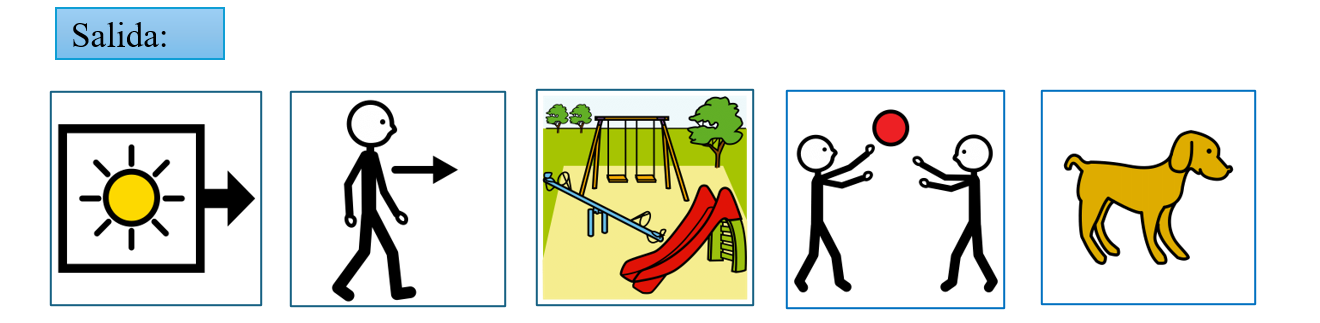
\includegraphics[width=0.75\textwidth]{img/ejemplo1.png}
    \caption{Ejemplo de secuencia de pictogramas}
    \label{fig:ejemplo de salida}
\end{figure}
El sistema no solo debe buscar las imágenes individuales que corresponden a cada palabra, sino sintetizar de forma óptima la estructura gramatical para presentar una secuencia coherente de pictogramas que mantenga la intención semántica original del usuario.

Las aproximaciones previas han abordado este reto bajo la premisa de que, para generar una secuencia de pictogramas coherente, primero es indispensable reducir la complejidad del lenguaje natural. Investigaciones como las de Cabello et al. \cite{cabello2018text} y Karmakar y Sinha \cite{karmakar-sinha-2024-aiding} introducen una estrategia que consiste en simplificar el texto de entrada al máximo, eliminando ambigüedades y estructuras gramaticales complejas, para después buscar los pictogramas que mejor representen esas unidades léxicas resultantes.

Con esta aproximación de simplificación y posterior correspondencia directa de palabras con pictogramas, se han consolidado las siguientes soluciones de software, las cuales son conocidas en el ámbito de la comunicación aumentativa y alternativa debido a su amplia adopción institucional. Como se resume en la Tabla \ref{tab:comparativa}, los sistemas actuales carecen de una comprensión profunda del contexto que constituye una oración.

\begin{table}[H]
\centering
\small
\begin{tabular}{|l|p{8cm}|p{2cm}|}
\hline
\textbf{Software} & \textbf{Enfoque y Limitaciones} & \textbf{Disponibilidad} \\ \hline
AraWord & \begin{itemize}[noitemsep, topsep=0pt]\item Relaciona directamente palabras o conceptos con pictogramas.
    \item Para procesar formas verbales mapea la conjugación a una tupla con el verbo en su forma base \autocite{perez2011}.
\end{itemize} & Open Source \\ \hline
Text-to-Pictogram  & \begin{itemize}[noitemsep, topsep=0pt]
\item Conecta palabras con unidades léxicas de WordNet para encontrar el pictograma más preciso.
\item Utiliza reglas específicas y diccionarios para palabras que no se encuentran en WordNet.
\item El sistema realiza un análisis lingüistíco por cada palabra individual, lo que causa que no se tome en cuenta el sentido global de la oración \autocite{vandeghinste2016}. 

\end{itemize} & Académico, Open Source \\ \hline
Aratraductor & \begin{itemize}[noitemsep, topsep=0pt]
    \item Identifica lemas y categorías gramaticales, eliminando elementos que no aportan significado visual como artículos y signos de puntuación \autocite{gervas2017}.
    \item Si no encuentra una palabra exacta busca su raíz para regresar siempre un pictograma,
    \item El sistema analiza grupo de palabras, para poder identificar palabras separadas que funcionan como una unidad léxica, como por ejemplo "crema solar", "sentido común", etc. 
\end{itemize} & Servicio Web Gratuito para integración \\ \hline
\end{tabular}
\caption{Comparativa de sistemas de traducción a pictogramas existentes.}
\label{tab:comparativa}
\end{table}

Frente a estas limitaciones, investigaciones recientes han demostrado que las arquitecturas basadas en Transformers pueden aprender mapeos complejos entre secuencias  sin depender de la construcción manual de recursos lingüísticos explícitos \cite{vaswani2017}. Al implementar modelos como T5 o mT5, que definen el estado del arte en tareas de generación de lenguaje natural \cite{raffel2020}, este trabajo propone dejar atrás los sistemas basados en reglas para adoptar un modelo  capaz de procesar el contexto de forma integral.


% \subsection{Métricas de evaluación}
% \label{sec:metricas}

% La evaluación automática de las secuencias de pictogramas generadas se realizará con tres métricas complementarias: \textbf{SacreBLEU}, \textbf{METEOR} y \textbf{Picto-term Error Rate (PictoER)}. Estas métricas comparan la hipótesis generada por el sistema (\texttt{hyp}) con la referencia anotada (\texttt{tgt}) y ofrecen señales diferentes sobre la calidad de la salida.

% \subsubsection{SacreBLEU}
% SacreBLEU es la implementación estandarizada de BLEU y mide la similitud entre la secuencia de pictogramas generada y la referencia mediante el conteo de \emph{n-gramas} coincidentes (usualmente hasta 4-gramas), incorporando una penalización por brevedad. La puntuación se expresa típicamente en una escala de 0 a 100, donde valores mayores indican mejor correspondencia. En la tarea ToPicto se emplea para garantizar consistencia en la evaluación entre participantes.

% \subsubsection{METEOR}
% METEOR es una métrica basada en alineamientos de unigramas que combina precisión y exhaustividad (\emph{recall}) mediante una medida $F$ ponderada, comúnmente definida como $F_{mean} = \frac{(1+\alpha)PR}{\alpha P + R}$, donde $\alpha$ suele tomar el valor 9 para dar mayor peso al \emph{recall}. Además, considera lemas, variaciones morfológicas y sinónimos, e incorpora una penalización por desorden (\emph{chunks}). La puntuación final se reporta en una escala de 0 a 100, donde valores más altos representan mejor desempeño.

% \subsubsection{Picto-term Error Rate (PictoER)}
% PictoER adapta el concepto de Word Error Rate al dominio de pictogramas, evaluando errores a nivel de tokens. Se calcula como $\text{PictoER} = \frac{S + D + I}{N} \times 100$, donde $S$ son sustituciones, $D$ eliminaciones, $I$ inserciones y $N$ el número total de tokens en la referencia. A diferencia de SacreBLEU y METEOR, valores más bajos indican mejor rendimiento, ya que representan menor cantidad de errores por token.


% \vspace{0.2cm}







% --- Otras secciones (Objetivo, Justificación, etc.) ---
\section{Objetivo}
Desarrollar un sistema de traducción automática de texto en lenguaje natural a secuencias de pictogramas ARASAAC, basado en arquitecturas de aprendizaje profundo (Transformers).

\textbf{Objetivos específicos:}

\begin{enumerate}
    \item Construir un corpus  Español-Pictogramas a partir de los datos de la tarea \textit{Text-to-Picto} de ImageCLEF 2026, realizando la traducción  y la validación de la alineación semántica para el idioma español.
    \item Implementar un modelo \textit{encoder-decoder} basado en Transformers para la tarea de traducción texto a pictogramas.
    \item Evaluar el sistema propuesto utilizando métricas estándar de traducción automática.
    \item Desarrollar una interfaz de usuario web que consuma el modelo entrenado mediante una API, permitiendo la interacción en tiempo real y la visualización de las secuencias generadas.

\end{enumerate}


\section{Justificación}

La comunicación constituye un derecho humano fundamental, sin embargo, su ejercicio pleno permanece inaccesible para las  personas que presentan discapacidades del lenguaje derivadas de condiciones como el autismo, la afasia, el síndrome de Rett o la parálisis cerebral. En México, el Instituto Nacional de Estadística y Geografía estima que más de más de 900 mil personas tienen una discapacidad para hablar o comunicarse \autocite{inegi2020cpv}, por tal motivo es relevante desarrollar herramientas tecnológicas de apoyo accesibles y eficaces. La Comunicación Aumentativa y Alternativa (CAA), particularmente mediante el uso de pictogramas, representa una de las vías más consolidadas para atender esta necesidad \autocite{beukelman2013}.

No obstante, los sistemas actuales de traducción automática de texto a pictogramas presentan limitaciones estructurales que restringen considerablemente su utilidad práctica. Herramientas como AraWord operan mediante mapeo léxico directo, ignorando el contexto de la oración \autocite{araword2020}. Por su parte,  Text-to-Pictogram incorpora redes léxicas y técnicas de desambiguación de sentidos, pero pierde la coherencia global al procesar el texto de forma lineal y modular \autocite{vandeghinste2016}. Otra herramienta para este propósito, Aratraductor, si bien dio un paso importante al usar análisis sintáctico  para identificar lemas y  usar una técnica de N-grams para detectar frases hechas; este enfoque depende demasiado de reglas gramaticales fijas, lo cual impide su generalización y escalabilidad. Ninguno de estos enfoques es capaz de modelar de forma integral las dependencias semánticas de una oración, tampoco de manejar adecuadamente fenómenos como la polisemia, la negación o las expresiones idiomáticas. La raíz de estas deficiencias reside en su arquitectura: al ser sistemas modulares basados en reglas o recursos lingüísticos explícitos, carecen de la capacidad de aprender representaciones contextuales a partir de datos.

Frente a este panorama, el presente trabajo propone una arquitectura de aprendizaje profundo unificada, fundamentado en la arquitectura Transformer \cite{vaswani2017}. A diferencia de los modelos precedentes, esta aproximación aprovecha el mecanismo de \textit{self-attention} para modelar dependencias globales en la oración, permitiendo que la generación de cada pictograma considere el contexto semántico completo y no solo la unidad léxica inmediata. La adopción de modelos pre-entrenados como T5 o mT5 \cite{raffel2020}  permite transferir conocimiento lingüístico profundo hacia la tarea específica de traducción a pictogramas. La originalidad de la propuesta reside en dos ejes: la aplicación de arquitecturas Transformer para el modelado integral del contexto, y la validación mediante un diseño experimental que emplea métricas estandarizadas de traducción automática. Esto permitirá realizar una comparativa objetiva entre el enfoque propuesto y los sistemas tradicionales basados en reglas.

El sistema beneficiaría directamente a personas usuarias de CAA y a sus familias, cuidadores y terapeutas del lenguaje, así como a desarrolladores de aplicaciones de accesibilidad, e incluso a personas aprendiendo un segundo idioma. Su viabilidad es alta,  por la disponibilidad abierta de los pictogramas ARASAAC, así como también por el aporte del corpus en inglés de la tarea \textit{Text-to-Picto} de ImageCLEF 2026. ImageCLEF es un laboratorio de evaluación internacional que forma parte de la CLEF (Conference and Labs of the Evaluation Forum), una iniciativa europea centrada en la evaluación de sistemas de información, se lleva a cabo cada año desde 2003 \autocite{unknown-author-no-date2}.

Desde una perspectiva académica, el proyecto abarca distintas áreas relevantes de la Ingeniería en Inteligencia Artificial. Lo anterior se logra al establecer un flujo de trabajo estructurado donde el procesamiento de lenguaje natural se usa para preparar los datos; luego apoyándose en el aprendizaje profundo, se entrena a un modelo Transformer, y finalmente las métricas de evaluación validan el éxito de los resultados. Al trabajar estas áreas como un conjunto unificado, el proyecto busca resultados técnicos confiables y un beneficio social real.
%============================================

% 4. PRODUCTOS O RESULTADOS ESPERADOS

% ============================================

% \section{Productos o Resultados Esperados}



% \begin{figure}[H]
% \centering
% \begin{tikzpicture}[
%     block/.style={rectangle, draw, minimum width=2.5cm, minimum height=1cm, align=center},
%     arrow/.style={->, thick}
% ]
%     % Bloques
%     \node[block] (input) at (0,0) {Texto\\(ES)};
%     \node[block] (encoder) at (4,0) {Encoder\\(Transformer)};
%     \node[block] (decoder) at (8,0) {Decoder\\(Transformer)};
%     \node[block] (output) at (12,0) {Secuencia de\\Pictogramas};  

%     % Flechas
%     \draw[arrow] (input) -- (encoder);
%     \draw[arrow] (encoder) -- (decoder);
%     \draw[arrow] (decoder) -- (output);

%     % Etiqueta
%     \node at (6,-1.5) {\textit{Arquitectura del sistema propuesto}};
% \end{tikzpicture}
% \caption{Diagrama de bloques del sistema de traducción texto-a-pictogramas.} 
% \label{fig:arquitectura}
% \end{figure}

\section{Productos o Resultados Esperados}

\begin{figure}[H]
\centering
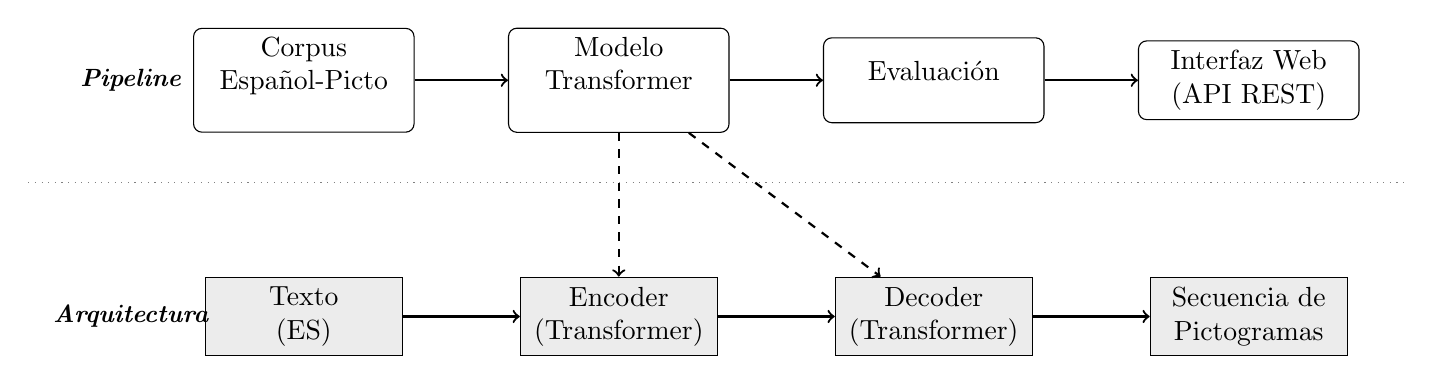
\begin{tikzpicture}[
    block/.style={rectangle, draw, minimum width=2.8cm, minimum height=1cm, align=center, rounded corners=3pt},
    blockmodel/.style={rectangle, draw, minimum width=2.5cm, minimum height=1cm, align=center, fill=gray!15},
    arrow/.style={->, thick},
    dashedarrow/.style={->, thick, dashed},
    label/.style={font=\small\itshape}
]

%% -------------------------------------------------------
%% NIVEL 1: Pipeline del proyecto (fila superior)
%% -------------------------------------------------------

\node[block] (corpus)   at (0, 3)   {Corpus\\Español-Picto\\};
\node[block] (modelo)   at (4, 3)   {Modelo\\Transformer\\};
\node[block] (eval)     at (8, 3)   {\\Evaluación\\};
\node[block] (web)      at (12, 3)  {Interfaz Web\\(API REST)};

\draw[arrow] (corpus) -- (modelo);
\draw[arrow] (modelo) -- (eval);
\draw[arrow] (eval)   -- (web);



%% -------------------------------------------------------
%% NIVEL 2: Arquitectura interna del modelo (fila inferior)
%% -------------------------------------------------------

\node[blockmodel] (input)   at (0, 0)  {Texto\\(ES)};
\node[blockmodel] (encoder) at (4, 0)  {Encoder\\(Transformer)};
\node[blockmodel] (decoder) at (8, 0)  {Decoder\\(Transformer)};
\node[blockmodel] (output)  at (12, 0) {Secuencia de\\Pictogramas};

\draw[arrow] (input)   -- (encoder);
\draw[arrow] (encoder) -- (decoder);
\draw[arrow] (decoder) -- (output);

% Conexión entre niveles (el bloque "modelo" del pipeline
% se corresponde con encoder+decoder abajo)
\draw[dashedarrow] (modelo) -- (encoder);
\draw[dashedarrow] (modelo) -- (decoder);

%% -------------------------------------------------------
%% Etiquetas de sección
%% -------------------------------------------------------
\node[label] at (-2.2, 3)   {\textbf{Pipeline}};
\node[label] at (-2.2, 0)   {\textbf{Arquitectura}};

% Línea divisoria opcional
\draw[dotted, gray] (-3.5, 1.7) -- (14, 1.7);

\end{tikzpicture}
\caption{Pipeline del proyecto y arquitectura interna del sistema de traducción texto-a-pictogramas. Las flechas punteadas indican la correspondencia entre el bloque de entrenamiento del pipeline y los componentes internos del modelo.}
\label{fig:arquitectura}
\end{figure}



\textbf{Productos esperados:}

\begin{enumerate}
    \item \textbf{Corpus paralelo Español-Pictogramas} Corpus paralelo Español-Pictogramas a partir de los datos de la tarea \textit{Text-to-Picto} de ImageCLEF 2026, realizando la traducción técnica y la validación de la alineación semántica para el idioma español.
    
    \item \textbf{Modelo entrenado:} Modelo entrenado para la tarea de traducción automática de español a pictogramas.

    \item \textbf{Aplicación web:} Implementación del modelo de traducción en un interfaz web para visualizar traducciones texto a pictograma. 

    \item \textbf{Documentación técnica:} Reporte técnico del trabajo terminal.

\end{enumerate}

\section{Metodología}

La metodología del proyecto seguirá de manera adaptada y práctica las fases del modelo \textit{CRISP-ML}, orientadas a garantizar calidad, trazabilidad y reproducibilidad en el desarrollo de un sistema de traducción automática de texto a pictogramas. Cada fase indica las actividades, entregables y controles de calidad asociados.

\begin{enumerate}

    \item \textbf{\textit{Business \& Data Understanding}}

    En una primera etapa, se definirá con claridad el problema desde una perspectiva técnica y social. Se establecerán los objetivos funcionales del sistema, determinando que el modelo deberá traducir texto en español a secuencias coherentes de pictogramas ARASAAC, preservando el significado semántico global del mensaje.

    Asimismo, se especificarán criterios de éxito medibles, tales como desempeño en métricas automáticas (\textit{SacreBLEU}, \textit{METEOR}, \textit{PictoER}), reducción de ambigüedades léxicas y tiempos de respuesta aceptables en la \textit{API} de inferencia. También se establecerán requisitos no funcionales relacionados con accesibilidad y reproducibilidad.

    \item \textbf{\textit{Data Engineering} (\textit{Data Preparation})}

    Se normalizarán los textos en español mediante procesos de limpieza, estandarización de caracteres y eliminación de inconsistencias tipográficas. Posteriormente, se aplicará una estrategia de tokenización adecuada para modelos \textit{Transformer}, posiblemente basada en sub-palabras.

    En paralelo, se definirá el vocabulario de salida correspondiente a los identificadores de pictogramas ARASAAC. Se estructurará el corpus en particiones de entrenamiento, validación y prueba, garantizando separación adecuada para evitar filtraciones de información.

    \item \textbf{\textit{Machine Learning Model Engineering}}

    En la fase de modelado se implementará un sistema basado en arquitecturas \textit{Transformer} de tipo \textit{encoder-decoder}. Se realizará el ajuste fino (\textit{fine-tuning}) de un modelo preentrenado como \textit{T5} o \textit{mT5}, adaptándolo a la tarea específica de traducción texto-a-pictogramas.

    Se establecerán configuraciones experimentales que incluirán selección de hiperparámetros, optimizador, tasa de aprendizaje y estrategias de regularización. Se utilizará validación temprana para prevenir sobreajuste y se almacenarán los pesos correspondientes a los mejores modelos obtenidos.
    
    Adicionalmente, se implementará un sistema base comparativo, posiblemente basado en mapeo léxico directo, con el fin de establecer una referencia cuantitativa que permita demostrar las mejoras aportadas por el enfoque neuronal.

    \item \textbf{\textit{Evaluating Machine Learning Models}}

    El sistema entrenado será evaluado utilizando métricas estándar de traducción automática como \textit{SacreBLEU}, \textit{METEOR} y \textit{PictoER}.

    Los resultados obtenidos se compararán sistemáticamente con los sistemas basados en reglas descritos en el estado del arte, estableciendo una discusión crítica sobre ventajas y limitaciones del enfoque propuesto.

    \item \textbf{\textit{Deployment}}

    Una vez validado el modelo, se procederá a su integración en una arquitectura de servicio. El modelo será encapsulado en una \textit{API REST} que permitirá recibir texto en español y devolver la secuencia correspondiente de pictogramas.

    Posteriormente, se desarrollará una interfaz web que consumirá dicha \textit{API}, permitiendo al usuario introducir texto y visualizar de forma inmediata los pictogramas generados. La interfaz priorizará criterios de accesibilidad y claridad visual, asegurando facilidad de uso para usuarios finales.
    
    El sistema será empaquetado mediante tecnologías de contenedorización, lo que permitirá su despliegue reproducible en distintos entornos.

    \item \textbf{\textit{Monitoring and Maintenance}}
    
    Se monitoreará el modelo durante un periodo determinado para verificar su correcto funcionamiento mediante el análisis de métricas de desempeño. En caso de detectar anomalías o degradación en el rendimiento, se realizará el mantenimiento correspondiente.

\end{enumerate}

% =========================
% Cronograma de Actividades (TDSP)
% =========================

\newpage
\section{Cronograma de Actividades (\textit{CRISP-ML})}

\subsection{Leyenda}
\noindent Las columnas representan los meses planificados (AGO..JUN). Cada actividad se encuentra alineada con las fases principales de la metodología \textit{CRISP-ML} y con las responsabilidades asignadas dentro del proyecto.

\subsection{Cronograma - Alumno: Naomi Isabel Robles Guzmán}
\begin{table}[H]
\centering\footnotesize
\begin{tabular}{|p{5.5cm}|c|c|c|c|c|c|c|c|c|c|c|}
\hline
\textbf{Actividad} & \textbf{AGO} & \textbf{SEP} & \textbf{OCT} & \textbf{NOV} & \textbf{DIC} & \textbf{ENE} & \textbf{FEB} & \textbf{MAR} & \textbf{ABR} & \textbf{MAY} & \textbf{JUN} \\ \hline

Investigación y análisis de arquitecturas técnicas utilizadas en trabajos similares. & \cellcolor{gris30} & \cellcolor{gris30} & & & & & & & & & \\ \hline

Definición de requisitos, criterios de éxito y análisis de viabilidad técnica. & \cellcolor{gris30} & \cellcolor{gris30} & & & & & & & & & \\ \hline

Traducción y validación del conjunto de datos proporcionado por ImageClef, adaptándolo al idioma español & & \cellcolor{gris30} & \cellcolor{gris30} & \cellcolor{gris30} & & & & & & & \\ \hline

Limpieza, estandarización y tokenización de datos para modelos \textit{Transformer}. & & & \cellcolor{gris30} & \cellcolor{gris30} & & & & & & & \\ \hline

Implementación de la arquitectura \textit{encoder-decoder} basada en \textit{Transformers}. & & & \cellcolor{gris30} & \cellcolor{gris30} & & & & & & & \\ \hline

Proceso de \textit{fine-tuning} y optimización de hiperparámetros del modelo. & & & & \cellcolor{gris30} & \cellcolor{gris30} & \cellcolor{gris30} & & & & & \\ \hline

Evaluación TT1 & & & & \cellcolor{gris30} & \cellcolor{gris30} & & & & & & \\ \hline

Evaluación con métricas automáticas (\textit{SacreBLEU}, \textit{METEOR} y \textit{PictoER}). & & & & & & & \cellcolor{gris30} & \cellcolor{gris30} & & & \\ \hline

Análisis comparativo contra sistemas basados en reglas . & & & & & & & & \cellcolor{gris30} & \cellcolor{gris30} & & \\ \hline

Diseño y desarrollo de la \textit{API REST} para el servicio de inferencia. & & & & & & & & & \cellcolor{gris30} & \cellcolor{gris30} & \\ \hline

Desarrollo de interfaz web y visualización de secuencias en tiempo real. & & & & & & & & & & \cellcolor{gris30} & \cellcolor{gris30} \\ \hline

Pruebas de integración, monitoreo de rendimiento y ajustes finales. & & & & & & & & & & & \cellcolor{gris30} \\ \hline

Redacción de documento técnico. & & & \cellcolor{gris30} & \cellcolor{gris30} & \cellcolor{gris30} & \cellcolor{gris30} & \cellcolor{gris30} & \cellcolor{gris30} & \cellcolor{gris30} & \cellcolor{gris30} & \\ \hline

Evaluación TT2 & & & & & & & & & & \cellcolor{gris30} & \cellcolor{gris30} \\ \hline
\end{tabular}
\end{table}

\subsection{Cronograma - Alumno: Ugalde Téllez Aarón}
\begin{table}[H]
\centering\footnotesize
\begin{tabular}{|p{5.5cm}|c|c|c|c|c|c|c|c|c|c|c|}
\hline
\textbf{Actividad} & \textbf{AGO} & \textbf{SEP} & \textbf{OCT} & \textbf{NOV} & \textbf{DIC} & \textbf{ENE} & \textbf{FEB} & \textbf{MAR} & \textbf{ABR} & \textbf{MAY} & \textbf{JUN} \\ \hline

Investigación y análisis de arquitecturas técnicas utilizadas en trabajos similares. & \cellcolor{gris30} & \cellcolor{gris30} & & & & & & & & & \\ \hline

Definición de requisitos, criterios de éxito y análisis de viabilidad técnica. & \cellcolor{gris30} & \cellcolor{gris30} & & & & & & & & & \\ \hline

Traducción y validación del conjunto de datos proporcionado por ImageClef, adaptándolo al idioma español & & \cellcolor{gris30} & \cellcolor{gris30} & \cellcolor{gris30} & & & & & & & \\ \hline

Limpieza, estandarización y tokenización de datos para modelos \textit{Transformer}. & & & \cellcolor{gris30} & \cellcolor{gris30} & & & & & & & \\ \hline

Implementación de la arquitectura \textit{encoder-decoder} basada en \textit{Transformers}. & & & \cellcolor{gris30} & \cellcolor{gris30} & & & & & & & \\ \hline

Proceso de \textit{fine-tuning} y optimización de hiperparámetros del modelo. & & & & \cellcolor{gris30} & \cellcolor{gris30} & \cellcolor{gris30} & & & & & \\ \hline

Evaluación TT1 & & & & \cellcolor{gris30} & \cellcolor{gris30} & & & & & & \\ \hline

Evaluación con métricas automáticas (\textit{SacreBLEU}, \textit{METEOR} y \textit{PictoER}). & & & & & & & \cellcolor{gris30} & \cellcolor{gris30} & & & \\ \hline

Análisis comparativo contra sistemas basados en reglas . & & & & & & & & \cellcolor{gris30} & \cellcolor{gris30} & & \\ \hline

Diseño y desarrollo de la \textit{API REST} para el servicio de inferencia. & & & & & & & & & \cellcolor{gris30} & \cellcolor{gris30} & \\ \hline

Desarrollo de interfaz web y visualización de secuencias en tiempo real. & & & & & & & & & & \cellcolor{gris30} & \cellcolor{gris30} \\ \hline

Pruebas de integración, monitoreo de rendimiento y ajustes finales. & & & & & & & & & & & \cellcolor{gris30} \\ \hline

Redacción de documento técnico. & & & \cellcolor{gris30} & \cellcolor{gris30} & \cellcolor{gris30} & \cellcolor{gris30} & \cellcolor{gris30} & \cellcolor{gris30} & \cellcolor{gris30} & \cellcolor{gris30} & \\ \hline

Evaluación TT2 & & & & & & & & & & \cellcolor{gris30} & \cellcolor{gris30} \\ \hline
\end{tabular}
\end{table}


% --- Referencias IEEE ---
\newpage
\begin{minipage}[t]{0.95\textwidth}
    \printbibliography[title={7. Referencias}]
\end{minipage}


% --- Sección 8: Alumnos y Directores ---
\newpage
\section{Alumnos y directores}

% Fila 1: Alumno 1 y Cuadro de Confidencialidad
\begin{minipage}[t]{0.52\textwidth}
    \textbf{Naomi Isabel Robles Guzmán.} Alumna de la carrera de Ing. en Inteligencia Artificial en ESCOM, Especialidad Inteligencia Artificial, Boleta: 2023630670, Tel. 5565088309, naomi.robguz@gmail.com. 
    
    \vspace{0.8cm}
    Firma: \rule{5cm}{0.4pt} 
\end{minipage}
\hfill
\begin{minipage}[t]{0.42\textwidth}
    \vspace{-0.5cm} % Ajuste para alinear con el título 8
    \begin{tcolorbox}[
        enhanced,
        sharp corners,
        colback=gray!30, % Fondo gris al 30% según CATT 
        colframe=black,
        boxrule=0.5pt,
        left=2pt, right=2pt, top=5pt, bottom=5pt,
        width=\textwidth,
        align=center
    ]
        \fontsize{8}{10}\selectfont
        \textbf{CARÁCTER:} Confidencial  \\
        \textbf{FUNDAMENTO LEGAL:} Artículo 11 Fracc. V y Artículos 108, 113 y 117 de la Ley Federal de Transparencia y Acceso a la Información Pública. \\
        \textbf{PARTES CONFIDENCIALES:} Número de boleta y teléfono.
    \end{tcolorbox}
\end{minipage}

\vspace{0.6cm}

% Fila 2: Alumno 2
\begin{minipage}[t]{0.55\textwidth}
    \textbf{Aarón Ugalde Téllez.} Alumno de la carrera de Ing. en Inteligencia Artificial en ESCOM, Especialidad Inteligencia Artificial, Boleta: 2023630739, Tel. 5541456229, aaronugaldet@gmail.com. 
    
    \vspace{0.8cm}
    Firma: \rule{5cm}{0.4pt}
\end{minipage}

\vspace{1cm}

% Fila 3: Director 1

\begin{minipage}[t]{0.55\textwidth}
    \textbf{Ana María Winfield Reyes. -} Doctora en Ciencias Administrativas por el Instituto Politécnico Nacional. Profesora de ESCOM/IPN. Áreas de Interés: educación, valores y escritura. Tel. 5729600 Ext. 52070, email: awinfieldr@ipn.mx
    
    \vspace{0.8cm}
    Firma: \rule{5cm}{0.4pt} 
\end{minipage}

\vspace{1cm}

% Fila 4: Director 2
\begin{minipage}[t]{0.55\textwidth}
    \textbf{Juan Irving Vásquez Gómez. -} Doctor en ciencias por el Instituto Nacional de Astrofísica, Óptica y Eletrónica (INAOE), 2014. Profesor titular en el Instituto Politécnico Nacional desde 2021. Áreas de interés: Aprendizaje profundo e inteligencia artificial. email: jvasquezg@ipn.mx
    
    \vspace{0.8cm}
    Firma: \rule{5cm}{0.4pt}
\end{minipage}

\end{document}